\chapter{Architecture Constraints}

\section{Environment}
\label{sec:Environment}
In the context of an AUTOSAR ECU, RTA-SUM modules are technically built as Application Software Components. Therefore, each RTA-SUM module requires a full AUTOSAR SW stack to run. We assume that the following AUTOSAR SW will be used:
\begin{longtable}{|l|l|l|}
\hline
\begin{minipage}{0.18\linewidth}\raggedright\vspace{.75ex}\textbf{Tool Name}\vspace{.75ex}\end{minipage} & \begin{minipage}{0.18\linewidth}\raggedright\vspace{.75ex}\textbf{Version}\vspace{.75ex}\end{minipage} & \begin{minipage}{0.55\linewidth}\raggedright\vspace{.75ex}\textbf{Description}\vspace{.75ex}\end{minipage}\\
\hline\hline
\endfirsthead
\hline
\begin{minipage}{0.18\linewidth}\raggedright\vspace{.75ex}\textbf{Tool Name}\vspace{.75ex}\end{minipage} & \begin{minipage}{0.18\linewidth}\raggedright\vspace{.75ex}\textbf{Version}\vspace{.75ex}\end{minipage} & \begin{minipage}{0.55\linewidth}\raggedright\vspace{.75ex}\textbf{Description}\vspace{.75ex}\end{minipage}\\
\hline\hline
\endhead
\hline
\endfoot
\hline
\endlastfoot
\begin{minipage}{0.18\linewidth}\raggedright\vspace{.75ex}ISOLAR-AB\vspace{.75ex}\end{minipage} & \begin{minipage}{0.18\linewidth}\raggedright\vspace{.75ex}12.3.3BETA1\vspace{.75ex}\end{minipage} & \begin{minipage}{0.55\linewidth}\raggedright\vspace{.75ex}AUTOSAR Authoring and BSW Configuration tools.\vspace{.75ex}\end{minipage}\\\hline
\begin{minipage}{0.18\linewidth}\raggedright\vspace{.75ex}RTA-BSW\vspace{.75ex}\end{minipage} & \begin{minipage}{0.18\linewidth}\raggedright\vspace{.75ex}12.3.3pr1\vspace{.75ex}\end{minipage} & \begin{minipage}{0.55\linewidth}\raggedright\vspace{.75ex}BSW automatic configuration and code generation.\vspace{.75ex}\end{minipage}\\\hline
\begin{minipage}{0.18\linewidth}\raggedright\vspace{.75ex}RTA-RTE\vspace{.75ex}\end{minipage} & \begin{minipage}{0.18\linewidth}\raggedright\vspace{.75ex}12.4.0\vspace{.75ex}\end{minipage} & \begin{minipage}{0.55\linewidth}\raggedright\vspace{.75ex}RTE generator used for testing\vspace{.75ex}\end{minipage}\\\hline
\begin{minipage}{0.18\linewidth}\raggedright\vspace{.75ex}RTA-OS\vspace{.75ex}\end{minipage} & \begin{minipage}{0.18\linewidth}\raggedright\vspace{.75ex}6.1.0\vspace{.75ex}\end{minipage} & \begin{minipage}{0.55\linewidth}\raggedright\vspace{.75ex}OS that is used for testing, as AUTOSAR OS\vspace{.75ex}\end{minipage}\\\hline
\begin{minipage}{0.18\linewidth}\raggedright\vspace{.75ex}MemMapGen\vspace{.75ex}\end{minipage} & \begin{minipage}{0.18\linewidth}\raggedright\vspace{.75ex}12.3.0\vspace{.75ex}\end{minipage} & \begin{minipage}{0.55\linewidth}\raggedright\vspace{.75ex} MemMap header file generator.\vspace{.75ex}\end{minipage}\\\hline
\begin{minipage}{0.18\linewidth}\raggedright\vspace{.75ex}Cantata\vspace{.75ex}\end{minipage} & \begin{minipage}{0.18\linewidth}\raggedright\vspace{.75ex}9.5\vspace{.75ex}\end{minipage} & \begin{minipage}{0.55\linewidth}\raggedright\vspace{.75ex}Used for functional testing\vspace{.75ex}\end{minipage}\\\hline
\end{longtable}

\section{Layers Definition}
The SUM\_SOH is a software module in the application layer of the standardized architecture of AUTOSAR (Figure~\ref{fig:Layers}). 
It interacts with other RTA-SUM modules and components of the BSW. In the latter case, the RTE is the means through which the interaction takes place.
\begin{figure}[htp]
\centering
	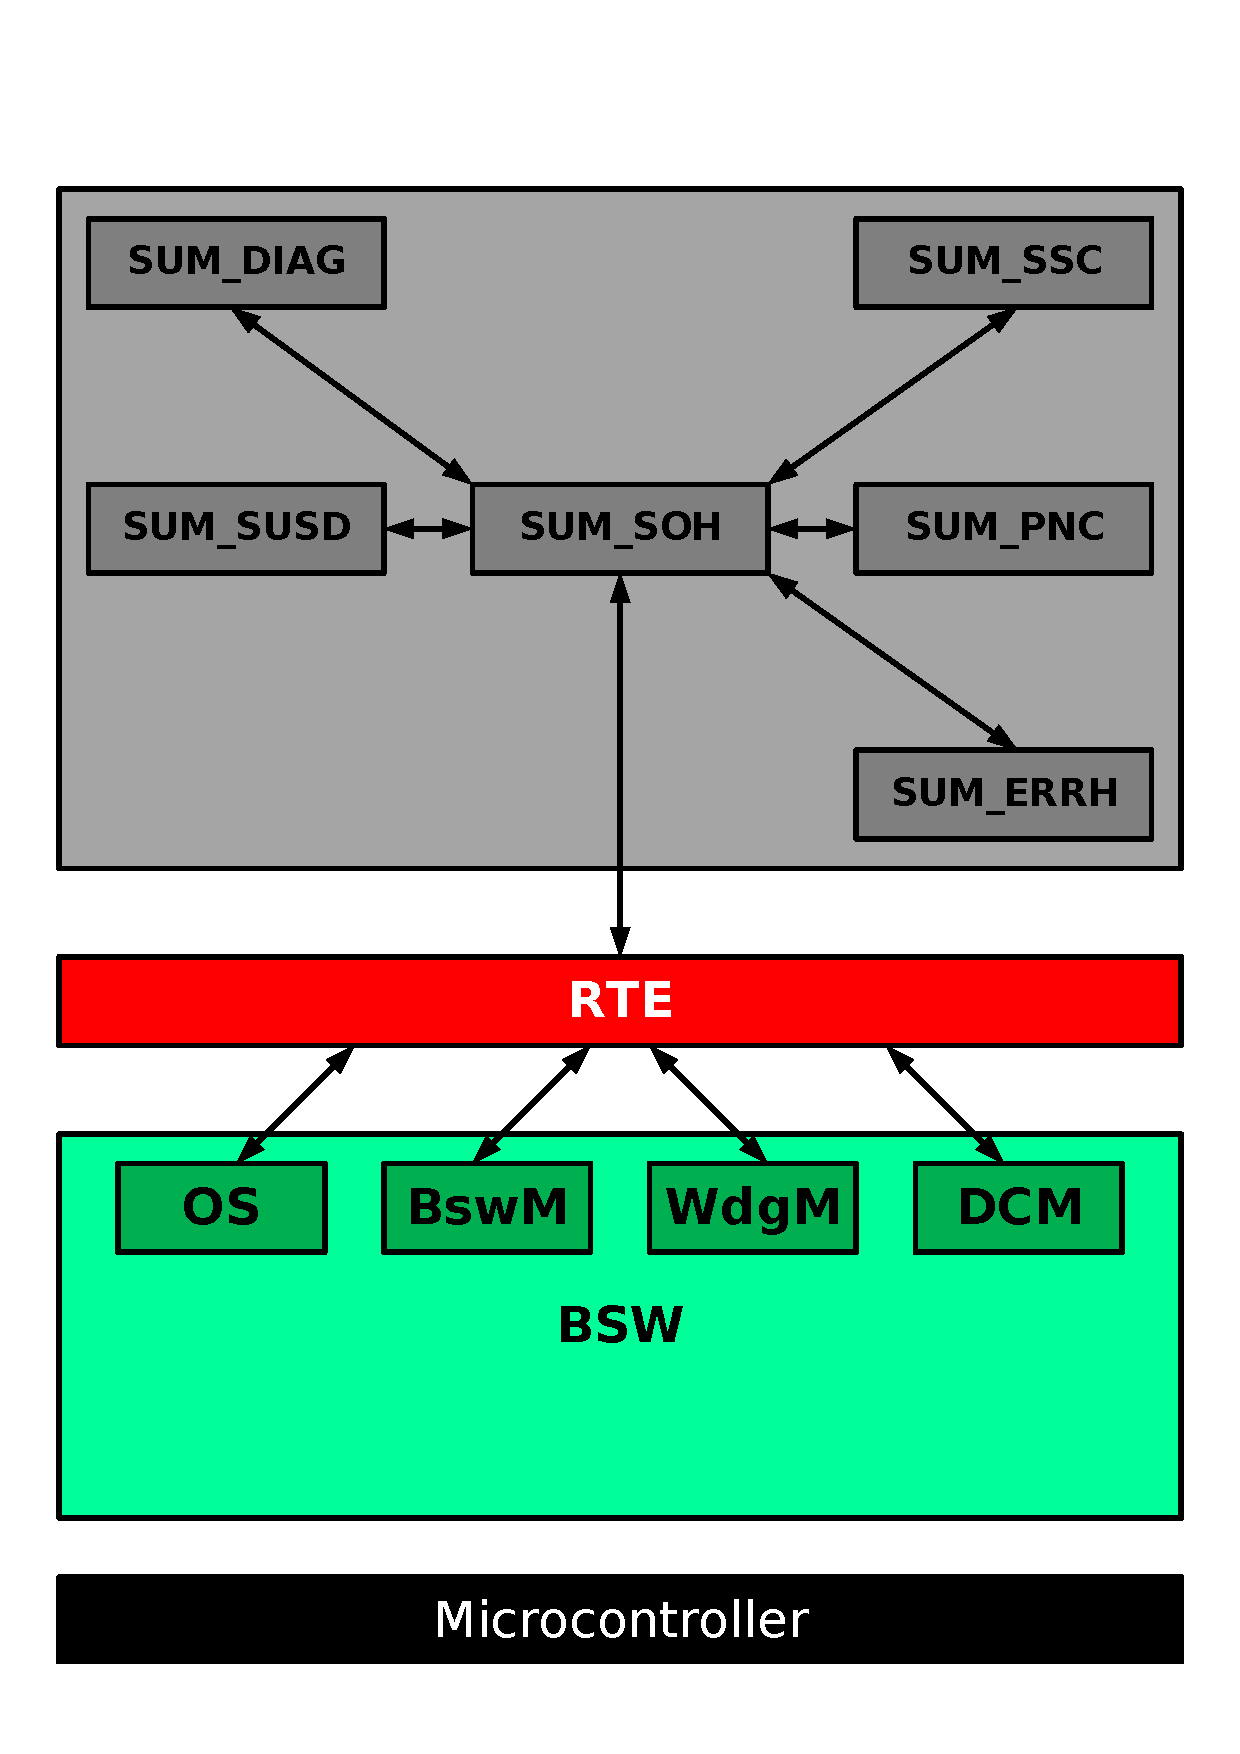
\includegraphics[scale=0.3]{images/Layers}
	\caption{System layer overview.}
	\label{fig:Layers}
\end{figure}

\section{Generic component interface}

The external interfaces of RTA-SUM module, and most of the interactions among SUM modules are specified in GM GB 8002.

\section{Other constraints and assumptions}

The ECU in which the SUM_SOH is implemented shall have a Secure cumulative NVM memory type, as defined in CTRS section 7.1.6, accessible to the SUM_SOH.
The ECU in which the SUM_SOH is implemented shall have NonClearedRAM memory type accessible to the SUM_SOH.
The ECU in which the SUM_SOH is implemented shall have an AdaptableNVM memory type accessible to the SUM_SOH.

The ECU initialization sequence shall be implemented such that any NVM needed for the SUM_SOH function is available prior to the SUM_SOH being initialized.

For ECUs that implement Memory Partitioning mechanisms, the SUM_SOH shall be implemented in the supervisory partition of the ECU software. Rationale: SUM_SOH must be in the trusted partition in order to interface with OS services. Supervisory partition is expected to include BSW Modules.

The SUM_SOH shall be implemented as a Supervised Entity of the Watchdog Manager.